\section{Handover Trees}

\begin{figure*}[h]
    \centering
    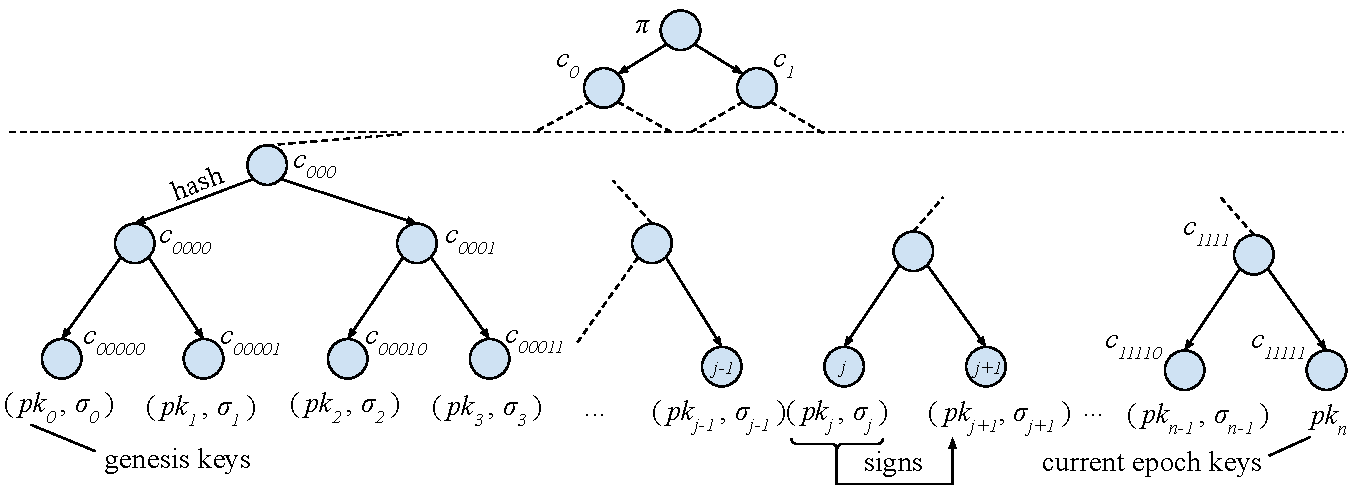
\includegraphics[width=0.8 \textwidth,keepaspectratio]{figures/popos-tree.pdf}
    \caption{The Proof of Proof-of-Stake tree, the central construction of our protocol.
             The root of the Merkle tree is the initial proof $\pi$. During the bisection
             game, the signatures between the challenge node $j$ and its neighbours
             $j-1$ and $j+1$ are validated.}
    \label{fig.popos-tree}
\end{figure*}

\import{./}{algorithms/alg.verifier}

The verifier requests from
the provers a Merkle Tree~\cite{merkle} commitment to the history of stake evolution of
the protocol. The provers send their respective commitments to the verifier. The verifier
then forwards the commitment of each prover to the other provers, allowing them to
challenge the statement of their peers. This challenge takes the form of a bisection
game, in which one path of the Merkle Tree is traversed until a leaf is reached.
When a leaf is reached, an adversarial prover will be discovered, as she will fail to provide
the required evidence of epoch transition. 
